\documentclass[a4paper]{IEEEtran}

\usepackage{xcolor}
\usepackage{hyperref}
\usepackage[utf8]{inputenc}
\usepackage[pdftex]{graphicx} 
\usepackage{multirow, pgfplotstable,booktabs,colortbl,lmodern}

\newcommand\TODO[1]{\textcolor{red}{TODO:#1}}
\newcommand\todo[1]{\TODO{#1}}
\newcommand\cn{\textcolor{red}{[citation needed]}}

\title{A Comparison of Delta Correlation Prefetchers}

\author{
    Sigve Sebastian Farstad,
    Rune Holmgren,
    Torbjørn Langland,
    Per Thomas Lundal
}

\begin{document}

\maketitle

\begin{abstract}
    This report examines the relative performances of different Delta Correlation prefetching schemes.
    Of the prefetchers tested, DCPT is shown experimentally to be the overall most performant prefetching scheme, but not by a land slide.

\end{abstract}

\section{Introduction}

This report is a solution to the mini-project for the course TDT4260 Computer Architecture at the Norwegian University of Science and Technology, spring 2014.
The assignment is to implement and evaluate the performance of one or more prefetchers. This report describes the implementation and test results done by group 11.

In this report, the relative performances of different Delta Correlation prefetchers is examined and discussed.

\section{Related Work}

\subsection{Delta Correlation Prefetching}

Delta Correlation Prefetching is a more advanced version of Stride Prefetching.
Stride Prefetching is based on identifying repeating memory address deltas.
The most recent delta along with some information describing its stability is stored and used to prefetch more cache lines.
The stability describes how many times the delta has repeated, and is used to determine how many cache lines to prefetch.
Programs such as those that use large arrays benefit greatly from Stride Prefetching, as they usually access memory in constant repeating intervals.

By storing a history of deltas instead of only the most recent, Data Correlation Prefetching is able to capture much more complex patterns than pure strides.
The history can then be searched for matches to the most recent deltas.
Each stored delta following the match would then be applied to the last address and prefethed.
It does however demand more storage space, which is proportional to the number of deltas.
Fig.~\ref{fig:delta_stream} shows a repeating pattern that can be captured by Delta Correlation but not with Stride Prefetching.
In the example, the two most recent deltas matches the first two, enabling a prefetch for address 31 and 40 to be issued.

\begin{figure}[!ht]
  \centering
      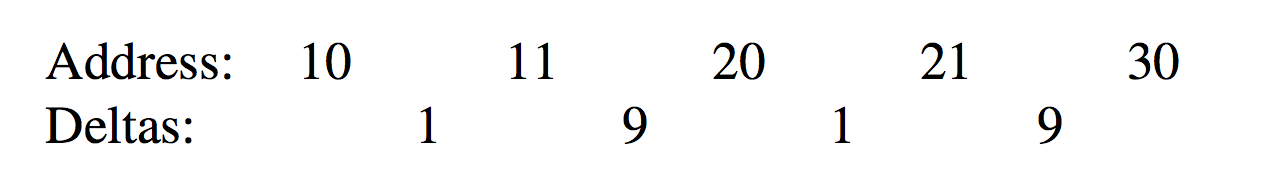
\includegraphics[width=0.4\textwidth]{Figures/DCExample}
  \caption{Example Delta Stream (Reprinted from \protect\cite{dcpt})}
  \label{fig:delta_stream}
\end{figure}

\subsection{Global History Buffer}

History based prefetchers need to store access patterns in efficient data structures that enable quick access.
One such data structure is the Global History Buffer (GHB) \cite{ghb} which is shown in Fig.~\ref{fig:ghb}.
GHB is an $n$-entry First-In, First-Out (FIFO) queue implemented as a circular buffer.
It stores the $n$ most recent L1 cache misses in entries that contain the miss address and a link pointer.
The link pointer is used to chain entries together into time-ordered linked lists that hold the significant access patterns.
An Index Table (IT) is used to keep track of these lists.
It maps some key to the most recent element of a linked list.
The IT is based on a FIFO queue like GHB, but significantly smaller as each entry has to be evaluated for each cache miss to look up a matching key.
The key can be based on any cache miss information, and depending on it a wide variety of history based prefetch methods can be implemented.

\begin{figure}[!ht]
  \centering
      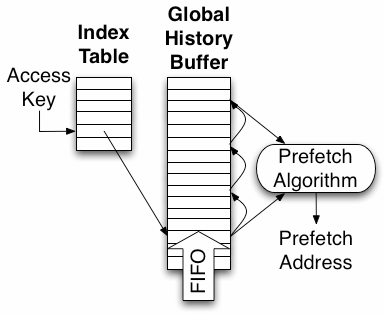
\includegraphics[width=0.4\textwidth]{Figures/ghb}
  \caption{Global History Buffer Structure (Reprinted from \protect{\cite{acdc}})}
  \label{fig:ghb}
\end{figure}

By keeping only recent data, it is not subject to any significant amount of stale data, and is better able to capture current access patterns.
Programs changing between several regular patterns may however not benefit from this, as one pattern might fill the whole buffer, causing information of the other to be lost.
In a comparison of different prefetch mechanisms by Péres et al.\cite{microlib}, one using GHB gave the best performance.

\section{Prefetcher Description}

Four different prefetchers are decribed in this section: CZone Delta Correlation, Program Counter Delta Correlation, Adaptive Program Counter Correlation and Delta Correlation Prediction Tables. 
All of the prefetchers are based on the common principle of Delta Correlation to detect memory access patterns, while three out of four use Global History Buffers for data storage.
Additionally all except one use the Program Counter of the load instruction at Index Table key.

\subsection{CZone Delta Correlation}

The concept of concentration zones (CZones) is based on the assumption that access within a data structure is fairly regular and that similar data structures lie within close proximity of each other in memory.
It works by dividing the memory into different regions, each assigned its own tag (most significant bits of the memory address).
Memory access patterns are then traced within these regions using Delta Correlation to determine prefetch candidates.

\begin{figure}[!ht]
  \centering
      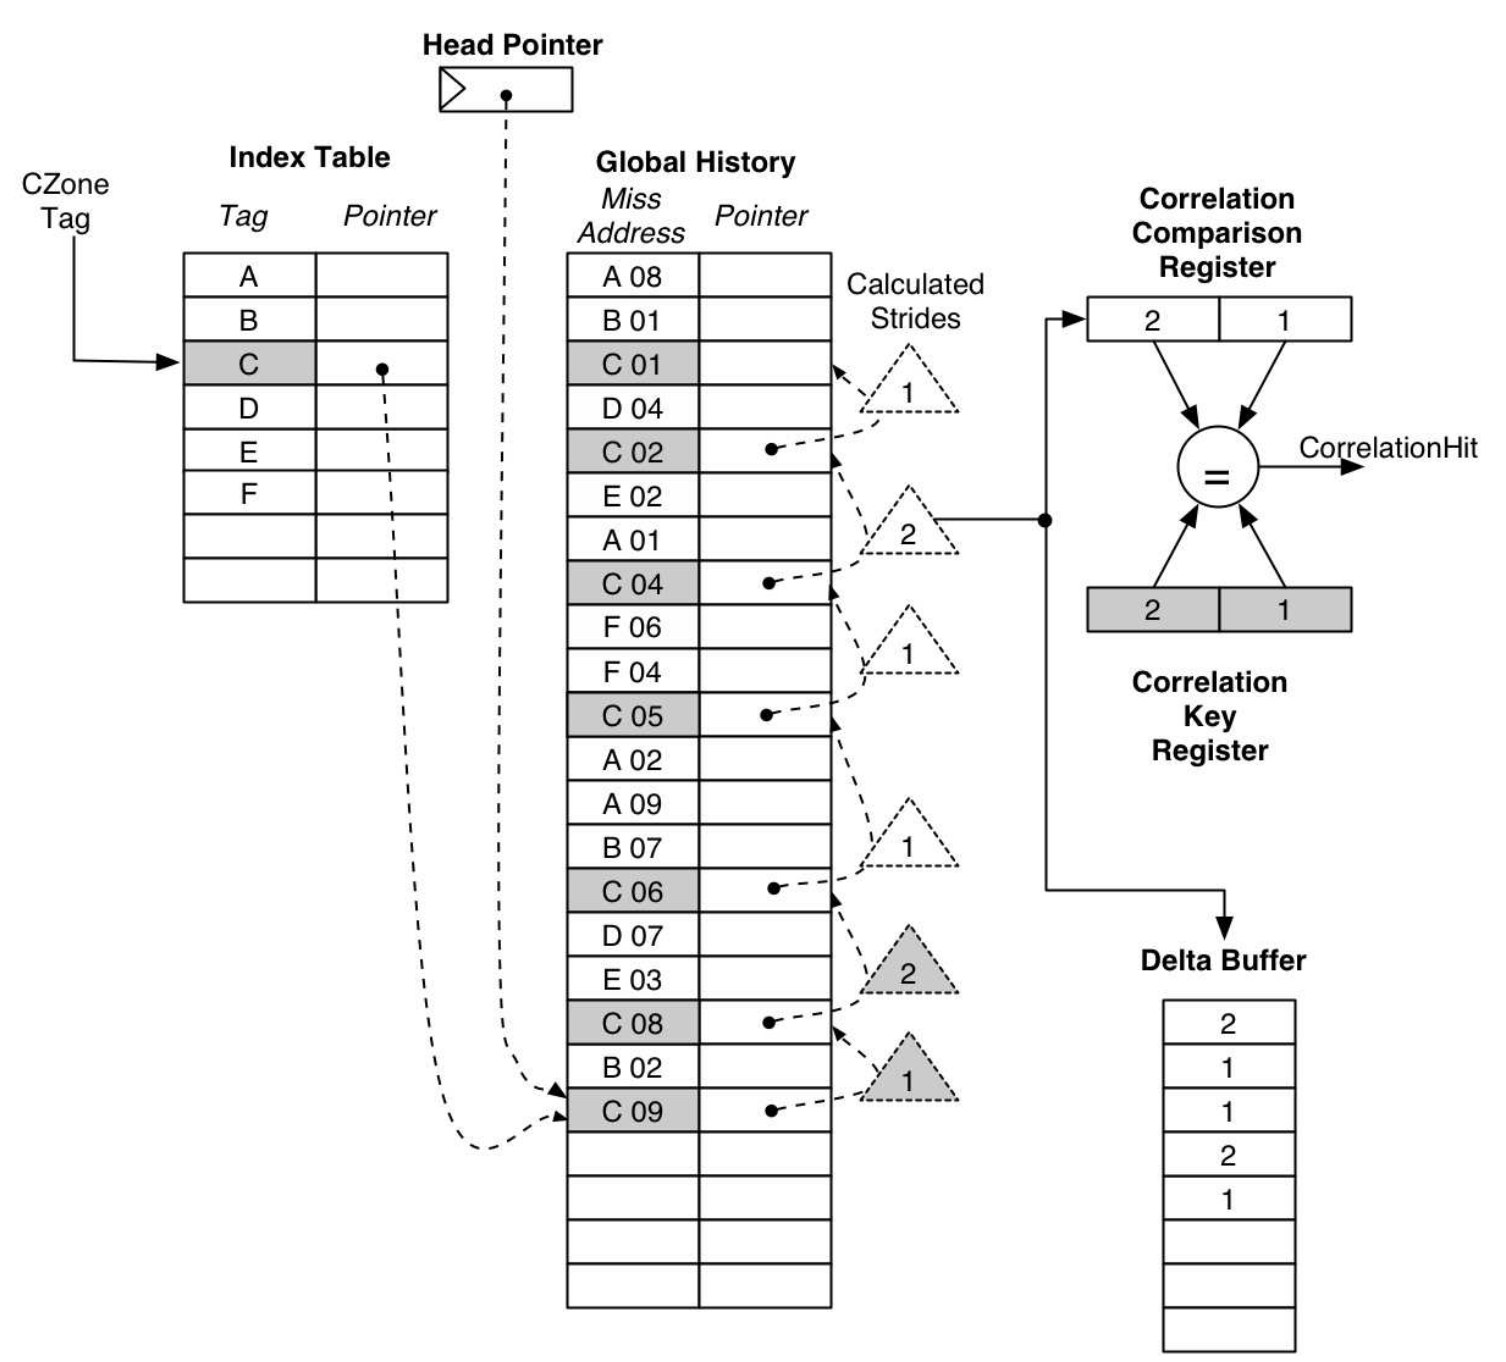
\includegraphics[width=0.5\textwidth]{Figures/CDC}
  \caption{CZone Delta Correlation (Reprinted from \protect\cite{acdc})}
  \label{fig:CDC}
\end{figure}

Fig.~\ref{fig:CDC} shows an example of a CZone Delta Correlation (CDC) Prefetcher that is implemented using GHB. 
Tag C from the index table points to address C09 from CZone C is the head, and is linked to C08,  which again is linked to C06, etc. 
The first two address deltas (1 and 2) from the linked list is added to the Correlation Key Register (2 and 1 in the example). 
The list is traversed, and the Correlation Comparison Register is continuously updated with the two latest deltas. 
When the correlation of the deltas of addresses C2-C4-C5 and C6-C8-C9  occurs, a delta buffer is filled with the deltas from the traversed list so far, and a prefetch based on the latest addresses and the deltas is issued.
Addresses C11, C12, C13, C15 and C16 will be calculated and prefetched.

\subsection{Program Counter Delta Correlation}

Program Counter Delta Correlation (PCDC) works in a similar way to CDC.
It uses the same data structures and correlation techniques, but differs in one key aspect; the IT key.
While CDC is based on the assumption that a program exhibits repeating access patterns within different sections of the memory, PCDC is based on the assumption that each load instruction exhibit repeating memory access patterns.
It is implemented by using the Program Counter (PC) of the load instruction as IT key instead of the memory region tag.

Programs where instructions repeat their access patterns within multiple memory regions, or where multiple instructions access different data structures within a single region interchangedly may benefit greatly from PCDC.

\subsection{Adaptive Program Counter Delta Correlation}

Different programs may respond differently to certain prefetching schemes, for some programs the response will be beneficial while negative for others due to trashing.
Thrashing is the term used to describe the effect of prefetching high amounts of unneeded cache lines, which requires eviction of those already in the cache that might be in frequent use.

The ability for a prefetcher to adapt to the programs' responses is greatly increases its potential.
When programs respond beneficialy, the prefetcher can increase its issue rate, while decreasing it or turning off prefetching all togethers when programs respond negatively.

Adaptivity is implemented by continuously recording and analysing the L2 cache hit rate, while the prefetcher experimentally evaluates different issue rates.
The best issue rate is then selected for a certain interval before the evaluation process is repeated.
This can be further improved by evaluating only the closest issue rate steps each time.

\subsection{Delta Correlation Prediction Tables}

Delta Correlation Prediction Tables (DCPT) can be seen as a slight variation of PCDC.
It was developed by Grannaes et al. \cite{dcpt} to reduce the amount of memory required to store delta information.
Instead of using a GHB to record the history, DCPT makes use of a table containing entries as seen in Fig.~\ref{fig:dcpt}.
Each entry contains  a field for the Program Counter (PC) identifying the instruction, the most recent memory address, the most recently prefetched address, and $n$ deltas in a circular buffer.

\begin{figure}[h!]
  \centering
      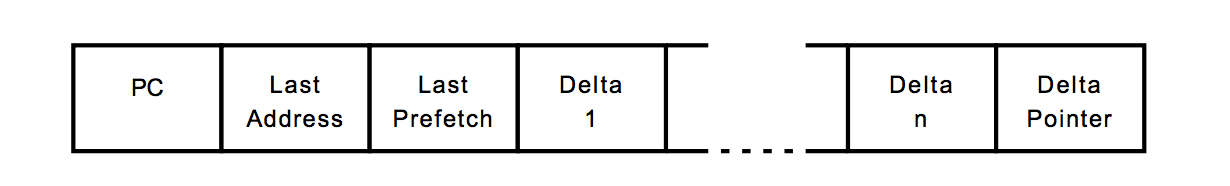
\includegraphics[width=0.5\textwidth]{Figures/DCTable}
  \caption{Delta Correlation Prediction Table (Reprinted from \protect\cite{dcpt})}
  \label{fig:dcpt}
\end{figure}

Short deltas are more common than long deltas in many programs.
This means that they often can be represented with very few bits while still capturing the patterns adequatly.
Since GHB must store the whole memory address and a link pointer at each access, while DCPT only stores a delta that may be a fraction of the size, this allows for more information to be stored in the same amount of space.
Additionally the deltas can be extracted directly without extra computation.

\section{Methodology}

In order to measure prefetcher performance, a test bench had to be made.
Software implementations of the different prefetcher behaviors were implemented nd simulated in a simulation framework.

\subsection{Simulation Framework}

A modified version of M5, the open-source TCP/IP network simulator\cite{M5paper}, has been used to simulate a hierarchical memory environment for evaluation of the different prefetcher implementations.
The modified M5 simulator is supplied as course material.

The memory model simulated by the framework is based on the Alpha 21264 microprocessor, which is a superscalar processor capable of out-of-order execution through speculative execution and instruction reordering.

The modified M5 user guide documents the exact architecture details:

\begin{quote}
The L1 prefetcher is split in a 32kB instruction cache, and a 64kB data cache.
Each cache block is 64B.
The L2 cache size is 1MB, also with a cache block size of 64B.
The L2 prefetcher is notified on every access to the L2 cache, both hits and misses.
There is no prefetching for the L1 cache.

The memory bus runs at 400MHz, is 64 bits wide, and has a latency of 30ns.~\cite{m5userguide}
\end{quote}

To simulate a prefetcher with the modified M5 framework, the behavior must be implemented as an M5 prefetcher module in C++ and plugged into the system.
To emulate realistic conditions for a hardware prefetcher implementation, a hard memory usage limit of 8KB was imposed on the software prefetchers.
That means that a prefetcher may only allocate up to 8KB of memory to hold any eventual data structures.
No further restrictions were imposed.

\subsection{SPEC CPU2000}

To measure the performances of the different prefetchers, the prefetchers were simulated and observed during runs against a subset of the SPEC CPU2000 benchmark suite.~\cite{http://dl.acm.org/citation.cfm?id=621510}

The benchmarks measure several key performance indicators:

\subsubsection{Speedup}
Speedup is the total execution speedup gained by using a given prefetcher compared to having no prefetcher at all.

\subsubsection{IPC}
IPC, or Instructions Per Cycle, measures how many instructions are executed per clock cycle of the processor.
Since the simulated M5 architecture is superscalar, this number can be greater than 1.

\subsubsection{Accuracy}
Accuracy is a measure that shows how many prefetches were useful.

\subsubsection{Coverage}
Coverage is a measurement that answers the question of how many potential prefetch candidates were identified by the prefetcher.

\subsubsection{Identified}
Identified is a measure that shows how many prefetches have been issued to the cache controller by the prefetcher.

\subsubsection{Issued}
Issued is a measure that shows how many prefetches have been issued to the next memory hierarchy level by the cache controller.

\subsection{PFJudge}

PFJudge is a prefetcher judge system available through an online web interface.
It is used in this project to run the M5-based simulations.

\subsection{Development}

The prefechers were developed in C using the M5 framework.
CDC and PCDC were developed as one prefetcher with a switch for toggling between the two modes, while APCDC implements an additional calibration function.
When a correlation is found, exactly the issue rate number of blocks are issued.
DCPT is based on the same prefetcher, but with GHB swapped out with DCPT.
It has no calibration function.

Experimentally, the best settings for CDC was found to be a issue rate of 1 and a tag size of 16 bits.
For PCDC the best issue rate was found to be 2, while for DCPT it was 3.
APCDC dynamicly adjusts the issue rate but has a maximum of 4.
Calibration is run in intervalls of 2048 cache misses, unless the best issue rate is determined to be the previous issue rate, in case it is extended to 16384 cache misses.
The IT size was 512 entries and GHB size was 1024 entries for all prefetchers using them, while DCPT table size was 180 entries containing 16 deltas of 16 bits each.
This results in no prefetcher using more than 8KB of memory for a hardware implementation, although the C program might reserve more to align values to words for increased execution speed.
Only the best of each kind has been taken into account in the comparison.

\section{Results}

The results from the benchmark runs are shown in Fig.~\ref{fig:results}.

\section{Discussion}

The first observation that can be made is that Delta Correlation prefetchers are generally more performant than simply using no prefetcher at all.
The exception to this is the CDC prefetcher, which is twice as slow as the other Delta Correlation prefetchers tested in the \texttt{ammp} test.
Indeed, it is even considerably worse than using no prefetcher at all.
The reason for this abysmal behavior can be seen in the accuracy statistics for the same test.
Where the other prefetchers have scored around 0.8 accuracy, which is quite good, CDC has scored less than one hundredth of that.
To have a prefetcher which is vulnerable to extremely poor performance in some secenarios is a bad idea, as it is at best inefficient, and at worst downright dangerous.
CDC is the only one of the tested prefetchers that have exhibited this kind of behavior.

\pgfplotstableread{
test_name        dcpt  apcdc cdc pcdc 
{ammp}           1.478 1.501 1   1
{applu}          1.088 1.077 1   1
{apsi}           1.037 1.010 1   1
{art110}         1.042 1.058 1   1
{art470}         1.042 1.058 1   1
{bzip2\_graphic} 1.145 1.067 1   1
{bzip2\_program} 1.035 1.040 1   1
{bzip2\_source}  1.004 1.006 1   1
{galgel}         1.040 1.082 1   1
{swim}           1.031 1.035 1   1
{twolf}          0.992 0.991 1   1
{wupwise}        1.226 1.238 1   1
}\speeduptable

\newcommand{\mgraph}[2]{
\begin{tikzpicture}[scale=0.5]
\begin{axis}[
  ybar, bar width=1pt,ymin=0,
  xmin=0.5,xmax=12.5, xtick=data,
  %axis y discontinuity=crunch,
  %ymin=0.75,
  xticklabels from table={#1}{test_name},
  xticklabel style={rotate=45,anchor=north east,inner sep=0mm},
  ylabel={\Large #2}, ylabel near ticks]
  \addplot table [x expr=\coordindex+1,y=dcpt] {#1};
  \addlegendentry{DCPT};
  \addplot table [x expr=\coordindex+1,y=apcdc] {#1};
  \addlegendentry{APCDC};
  \addplot table [x expr=\coordindex+1,y=cdc] {#1};
  \addlegendentry{CDC};
  \addplot table [x expr=\coordindex+1,y=pcdc] {#1};
  \addlegendentry{PCDC};
\end{axis}
\end{tikzpicture}
}

\newcommand{\mtable}[2]{
\centering
\resizebox{.81\columnwidth}{!}{
\pgfplotstabletypesetfile[
columns={test_name, dcpt, apcdc, cdc, pcdc},
every even row/.style={before row={\rowcolor{blue!15}}},
every head row/.style={
  before row={\toprule 
    \multirow{2}{*}{\bfseries Test Name} & \multicolumn{4}{c}{\bfseries #2}\\ \cmidrule{2-5}},
  after row=\midrule},
every last row/.style={after row=\bottomrule},
every row/.style={font=\tiny},
columns/test_name/.style={
  column name={},
  column type={l},
  string type},
columns/dcpt/.style={
  column name={DCPT},
  },
columns/apcdc/.style={
  column name={APCDC},
  },
columns/cdc/.style={
  column name={CDC},
  },
columns/pcdc/.style={
  column name={PCDC},
  },
    ] 
  {#1}
}
}


\pgfplotstableread{
test_name        dcpt  apcdc cdc pcdc 
{ammp}           1.478 1.501 1   1
{applu}          1.088 1.077 1   1
{apsi}           1.037 1.010 1   1
{art110}         1.042 1.058 1   1
{art470}         1.042 1.058 1   1
{bzip2\_graphic} 1.145 1.067 1   1
{bzip2\_program} 1.035 1.040 1   1
{bzip2\_source}  1.004 1.006 1   1
{galgel}         1.040 1.082 1   1
{swim}           1.031 1.035 1   1
{twolf}          0.992 0.991 1   1
{wupwise}        1.226 1.238 1   1
}\speeduptable
\pgfplotstableread{
test_name        dcpt  apcdc cdc pcdc 
{ammp}           0.122 0.124 1   1
{applu}          0.561 0.556 1   1
{apsi}           1.542 1.502 1   1
{art110}         0.127 0.129 1   1
{art470}         0.127 0.129 1   1
{bzip2\_graphic} 1.508 1.405 1   1
{bzip2\_program} 1.536 1.543 1   1
{bzip2\_source}  1.717 1.720 1   1
{galgel}         0.462 0.481 1   1
{swim}           0.705 0.708 1   1
{twolf}          0.421 0.420 1   1
{wupwise}        0.918 0.926 1   1
}\ipctable
\pgfplotstableread{
test_name        dcpt  apcdc cdc pcdc 
{ammp}           0.813 0.774 1   1
{applu}          0.636 0.525 1   1
{apsi}           0.403 0.355 1   1
{art110}         0.801 0.795 1   1
{art470}         0.801 0.795 1   1
{bzip2\_graphic} 0.896 0.788 1   1
{bzip2\_program} 0.807 0.574 1   1
{bzip2\_source}  0.782 0.702 1   1
{galgel}         0.655 0.739 1   1
{swim}           0.582 0.554 1   1
{twolf}          0.323 0.287 1   1
{wupwise}        0.667 0.667 1   1
}\accuracytable
\pgfplotstableread{
test_name        dcpt  apcdc cdc pcdc 
{ammp}           0.702 0.698 1   1
{applu}          0.332 0.336 1   1
{apsi}           0.173 0.028 1   1
{art110}         0.170 0.201 1   1
{art470}         0.170 0.201 1   1
{bzip2\_graphic} 0.755 0.577 1   1
{bzip2\_program} 0.537 0.229 1   1
{bzip2\_source}  0.625 0.459 1   1
{galgel}         0.425 0.924 1   1
{swim}           0.417 0.413 1   1
{twolf}          0.039 0.049 1   1
{wupwise}        0.667 0.651 1   1
}\coveragetable
\pgfplotstableread{
test_name        dcpt     apcdc    cdc pcdc 
{ammp}           13341801 19803635 1   1
{applu}          3243298  5414227  1   1
{apsi}           101119   16347    1   1
{art110}         14370198 54897828 1   1
{art470}         14370198 54897828 1   1
{bzip2\_graphic} 87717    72885    1   1
{bzip2\_program} 39751    23534    1   1
{bzip2\_source}  28729    23115    1   1
{galgel}         344166   781365   1   1
{swim}           2333012  4918637  1   1
{twolf}          156782   190970   1   1
{wupwise}        691877   551276   1   1
}\identifiedtable
\pgfplotstableread{
test_name        dcpt     apcdc     cdc pcdc 
{ammp}           12018716 112550456 1   1
{applu}          1160488  11423496  1   1
{apsi}           51421    19410     1   1
{art110}         2908765  13478208  1   1
{art470}         2908765  13478208  1   1
{bzip2\_graphic} 78988    168654    1   1
{bzip2\_program} 36835    122088    1   1
{bzip2\_source}  26851    122016    1   1
{galgel}         212199   1408948   1   1
{swim}           1622021  11688313  1   1
{twolf}          122898   1174298   1   1
{wupwise}        433846   1423433   1   1
}\issuedtable


\clearpage
\begin{figure*}[H]
\mgraph{\speeduptable}{Speedup}
\mgraph{\ipctable}{IPC}
\mgraph{\accuracytable}{Accuracy}
\mgraph{\coveragetable}{Coverage}
\mgraph{\identifiedtable}{Identified}
\mgraph{\issuedtable}{Issued}
\end{figure*}
\begin{figure*}[H]
\mtable{\speeduptable}{Speedup}
\mtable{\ipctable}{IPC}
\mtable{\accuracytable}{Accuracy}
\mtable{\coveragetable}{Coverage}
\mtable{\identifiedtable}{Identified}
\mtable{\issuedtable}{Issued}
\end{figure*}
\clearpage


\pgfplotstableread{
test_name  dcpt   apcdc pcdc  cdc   no_prefetcher
{}         1.0841 1.083 1.071 0.989 1.0
}\averagespeeduptable

\newcommand{\ngraph}[2]{
\begin{tikzpicture}[scale=0.5]
\begin{axis}[
  ybar, bar width=15pt,ymin=0,
  xmin=0.1,xmax=4, xtick=data,
  axis y discontinuity=crunch,
  ymin=0.9,
  xticklabels from table={#1}{test_name},
  xticklabel style={rotate=45,anchor=north east,inner sep=0mm},
  ylabel={\Large #2}, ylabel near ticks]
  \addplot table [x expr=\coordindex+1,y=dcpt] {#1};
  \addlegendentry{DCPT};
  \addplot table [x expr=\coordindex+1,y=apcdc] {#1};
  \addlegendentry{APCDC};
  \addplot table [x expr=\coordindex+1,y=cdc] {#1};
  \addlegendentry{CDC};
  \addplot table [x expr=\coordindex+1,y=pcdc] {#1};
  \addlegendentry{PCDC};
  \addplot table [x expr=\coordindex+1,y=no_prefetcher] {#1};
  \addlegendentry{No Prefetcher};
\end{axis}
\end{tikzpicture}
}
\begin{figure}[ht]
\centering
\ngraph{\averagespeeduptable}{Average speedup}
\caption{Average speedup}
\label{fig:speedup}
\end{figure}

% dcpc Blast #1 http://dm-ark.idi.ntnu.no/pf/184/details/
% apcdc APCDC#2 http://dm-ark.idi.ntnu.no/pf/166/details/
% cdc cdc-1-16 http://dm-ark.idi.ntnu.no/pf/1442/details/
% pcdc pcdc-2 http://dm-ark.idi.ntnu.no/pf/1447/details/


Other than the extreme discrepancy in the CDC \texttt{amms} test, there are not a lot of big differences.
Some tests favor one pretching scheme, while other tests favor another.
Overall, DCPT scores best on average with APCDC and PCDC on close second and third, as seen in Fig.~\ref{fig:speedup}.
Which one should be chosen over the other for use in a given real life application, however, largely depends on the characteristics of the application.

\todo{ Mention what could have been done better or different? Future ideas? }

\section{Conclusion}

In conclusion, while Delta Correlation based prefetching approaches are promising in general, there are some significant differences between the prefetching schemes tested.
The differences are however not uniformly in favor of a single prefetching scheme.
The benchmarks rather favor different schemes for different tests.

Looking at the average speedup though, DCPT emerges as the most performant scheme, closely followed by APCDC and PCDC, while CDC is the least performant scheme.


\bibliography{bibliography}
\bibliographystyle{plain}
\nocite{*}

\begin{IEEEbiography}[{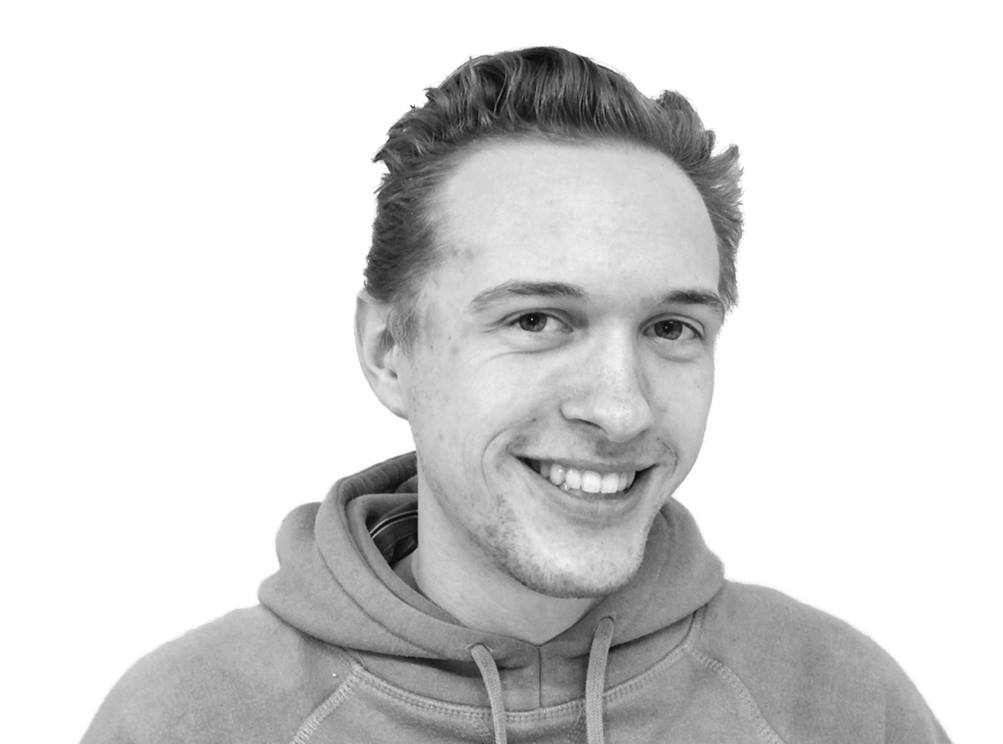
\includegraphics[width=1in,height=1.25in,clip,keepaspectratio]{Figures/farstad.jpg}}]{Sigve Sebastian Farstad}
    was born in Trondheim, Norway, in 1990.
    He is currently working towards an M.S. degree in computer science from the Norwegian University of Science and Technology, Trondheim, expecting to graduate in 2015.

    In 2009 he served as a civilian guardian of the Norwegian People, and he has since then worked as, amongst other things, a Software Consultant, a Technical Innovator in the mobile banking sector, a Professional Translator, and is currently working as one of the technical Co-Founders of feat.fm.

    Mr. Farstad was, together with other team members of the demo crew Ninjadev, the winner of the Web Demo Compo at Solskogen 2012.
\end{IEEEbiography}

\begin{IEEEbiography}[{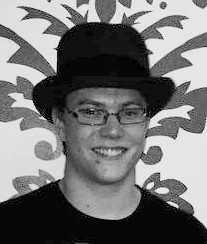
\includegraphics[width=1in,height=1.25in,clip,keepaspectratio]{Figures/holmgren.jpg}}]{Rune Holmgren}
    was born in Harstad, Norway, in 1991.
    He is currently working towards an M.S. degree in computer science from the Norwegian University of Science and Technology, Trondheim, expecting to graduate in 2015.

    He has worked as a Dairy Product Quality Assurance Intern, a Teaching Assistant for and most recently held the position of Summer Intern at Connome.

    Mr. Holmgren was recipient of the award Friidrettens Venners Kretspris in 2010.
\end{IEEEbiography}

\begin{IEEEbiography}[{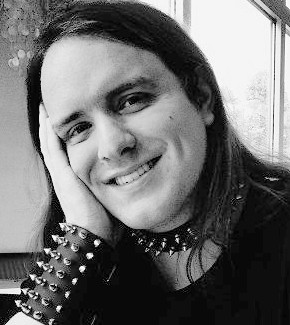
\includegraphics[width=1in,height=1.25in,clip,keepaspectratio]{Figures/langland.jpg}}]{Torbjørn Langland}
    was born in Trondheim, Norway, in 1987.
    He is currently working towards an M.S. degree in computer science from the Norwegian University of Science and Technology, Trondheim, expecting to graduate in 2015.

    He was worked as a Temporary Store Clerk and until recently held the title of Software Engineer at Comsol.

    Mr Langland is exceptionally good at playing Mario Kart 64.
\end{IEEEbiography}

\begin{IEEEbiography}[{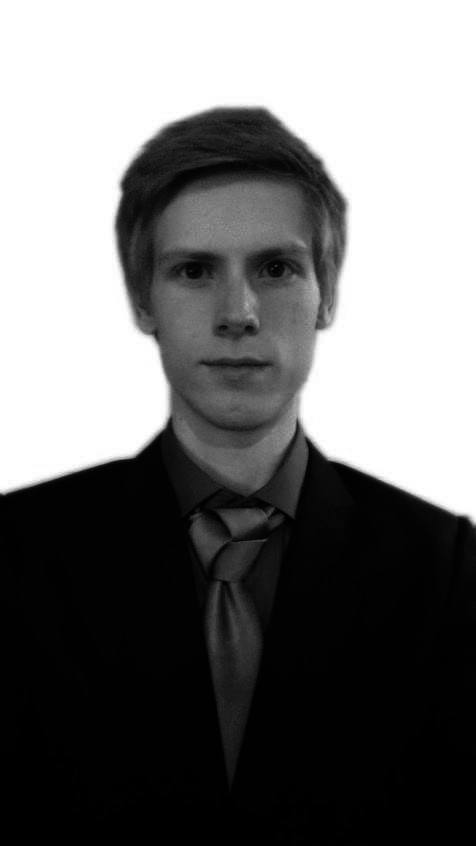
\includegraphics[width=1in,height=1.25in,clip,keepaspectratio]{Figures/lundal.jpg}}]{Per Thomas Lundal}
    was born in Trondheim, Norway, in 1991.
    He is currently working towards an M.S. degree in computer science from the Norwegian University of Science and Technology, Trondheim, expecting to graduate in 2015.

    He has since 2006 worked as a Sales Representative at Biltema.
    He has also worked as a Teaching Assistant for the course Programming Languages at NTNU.

    Mr. Lundal was the recipient of the Champions' Award and the Programming Award at the First Lego League, Trondheim.
\end{IEEEbiography}

\end{document}
